In this section, we present our measurement methodology along with the
metrics considered and discuss about the performance-power-energy trade-off of the model system on the different platforms stated.

\subsection{Measurement methodology}
\label{subsec:4.1}

We  approach  the  assessment  of  the energy  footprint  and  overall
performance   of   \cosmoart   with  two   important  metrics:
\textit{time-to-solution} (TTS) and \textit{energy-to-solution} (ETS).
TTS refers to  the total wall clock time  of the application execution
time. ETS  is the amount of  energy spent to  achieve results.  Energy
consumption  is  assessed by  sampling  the  power during execution which is then averaged and multiplied  by the TTS to determine  ETS. Whenever  possible,  multiple production  runs  were
performed  to  illustrate the  reproducibility  of  the baseline,  and
quantify the  significant uncertainties  in the power  measurement, as
dictated by the available technology.

For the experiments with \tinto platform, we also analyze the contribution of the MPI library to the energy consumption and how the use of the blocking versus polling message-passing policies can potentially render energy savings. Specifically, the OpenMPI 1.6.5 library, 
features two operation modes, blocking and polling, which can be selected before \cosmoart
is launched. In the polling configuration (the default mode) ``MPI'' continually polls
the network interface to check for the completion of an event (e.g. send or receive).
This usually yields low latency but high CPU utilization. Thus, one can expect that this mode 
attains the best performance, possibly at the cost a higher energy usage. In the blocking
mode, the CPU is yield to other processes/threads if there are no incoming messages.

\subsection{Time-power-energy analysis of \cosmoart}
\label{subsec:4.2}

\begin{figure}[htbf]
  \begin{center}
    \includegraphics[width=0.48\textwidth]{Figs/NRJ_benchmark_Monch.eps}
    \caption{\monch: Isola E1 Rack 2 Total Power.}
    \label{fig:1}
  \end{center}
\end{figure}

\begin{figure}[htbf]
  \begin{center}
    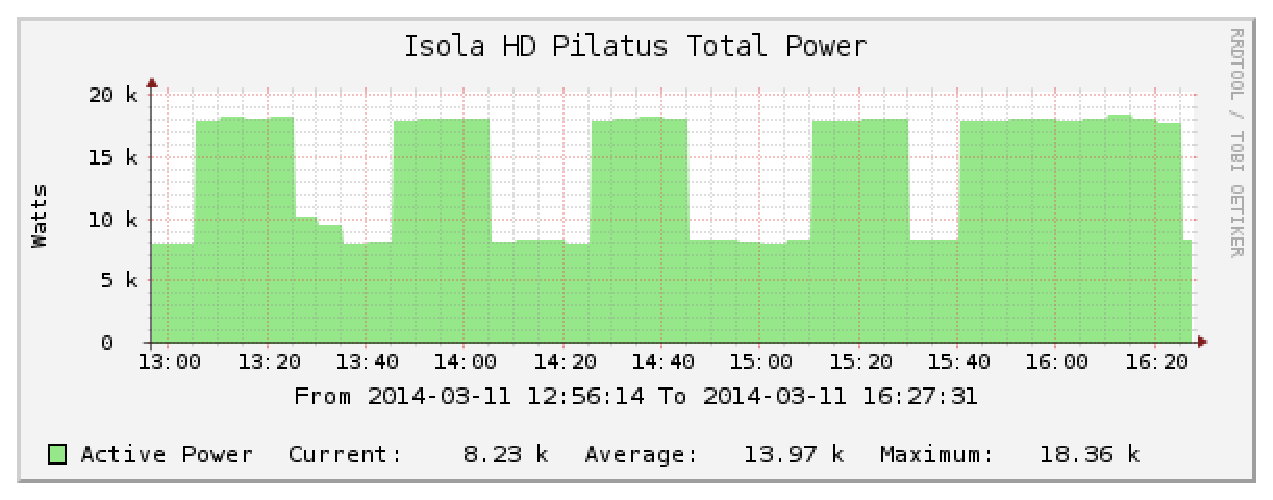
\includegraphics[width=0.48\textwidth]{Figs/NRJ_benchmark_Pilatus.eps}
    \caption{\pilat: Isola HD Total Power.}
    \label{fig:2}
  \end{center}
\end{figure}

Figures~\ref{fig:1}   and   \ref{fig:2}   account   respectively   for
\monch's Isola E1 Rack  2 and \pilat' Isola HD total
power measurements for  1-day or 2-day simulations. On  the Intel Ivy
Bridge EP  based cluster (i.e.  \monch),  the 1-day simulation
was issued  only twice due  to usage restrictions. As  time resolution
was set to one update every  5 minutes for power sampling, the average
power consumption was computed by considering 6 values for each single
run.  On the Intel Xeon E5 based cluster (i.e.  \pilat), the
1-day simulation  was issued  four times and  a 2-day run  only once.
Similarly, the average power consumption was computed by considering 4
values  for  each  single  1-day  run  and 9  values  for  the  2-days
run. Corresponding results are gathered in Table~\ref{tab:3}.

\begin{table}[htbf]
  \begin{center}
    \caption{Average power consumption (W) of the platforms}
    \label{tab:3}
    \begin{tabular}{cccc}
      \hline\noalign{\smallskip}
      \textbf{\scriptsize{Xeon E5}} & \textbf{\scriptsize{Ivy Bridge}} & \textbf{\scriptsize{Xeon  E5645}} & \textbf{\scriptsize{Xeon  E5645}}\\
      & & \textbf{\scriptsize{(Polling)}} & \textbf{\scriptsize{(Blocking)}} \\
      \noalign{\smallskip}\hline\noalign{\smallskip}
      18035.0 & 12622.5 & 3713.6 & 3651.8 \\ 
      \noalign{\smallskip}\hline
    \end{tabular}
  \end{center}
\end{table}

In  Figure~\ref{fig:3}, we  compare both  TTS (right  Y-axis)  and ETS
(left  Y-axis)  metrics  on  both  platforms.  As  expected,  Xeon  E5
outperforms Ivy Bridge EP, being  roughly 130\,\% faster.  The reason for
that is  two-fold: \emph{i}) it has  higher clock frequency  than Ivy Bridge
(2.6\,GHz  against  2.2\,GHz),  and  \emph{ii})  it  aims at  computing  speed
regardless to  energy consumption.  In our experiments,  Ivy Bridge EP
showed the best energy-to-solution, reducing the energy consumption of
Xeon E5 by approximately 7\,\%.

Averaged TTS and ETS results over 10 repetitions of 24h simulation on \tinto are shown in Figure~\ref{fig:4}. Correponding results for average total power are shown in Table~\ref{tab:3}.  
As expected, the average total power dissipated by \cosmoart while using the blocking MPI policy is about 2\,\% less than that consumed by the polling policy. This is due to the power-friendly (blocking) waits performed by the CPU cores while using the blocking MPI mode, in contrast to the polling waits that take place when the polling MPI mode is set. From the point of view of the execution time, there is a slight reduction for the blocking MPI mode. One can expect that the costs of the interruptions used in the blocking MPI policy can lead to an increase of the total execution time, however, applications with extensive computing, as e.g. \cosmoart, may show better performance with the blocking modes. This effect works in favor with our results since the energy consumed is also reduced (2\,\%) just by changing the behavior of the OpenMPI library to the blocking policy, i.e, with the \texttt{--mca mpi\_yield\_when\_idle} parameter set in the \texttt{mpirun} command.

\begin{figure}[htbf]
  \includegraphics[width=0.5\textwidth]{Figs/Time_E2S_COSMO-ART-0.eps}
  \caption{Time-to-solution and energy-to-solution comparison between
    Xeon E5 and Ivy Bridge-EP architectures for a 24h simulation.}
  \label{fig:3}
\end{figure}

\begin{figure}[htbf]
  \includegraphics[width=0.5\textwidth]{Figs/Time_E2S_COSMO-ART-5.eps}
  \caption{Mean time-to-solution and energy-to-solution on
    \tinto for a 24h simulation using the polling and blocking MPI policies. The 95\,\% confidence intervals of Student's $t$ distribution (10 samples) clearly indicates 
    an improvement for blocking policy in both TTS and ETS.}
  \label{fig:4}
\end{figure}

\subsection{Power-performance tracing on \tinto}
\label{subsec:4.3}

A full tracing experiment is conducted on \tinto in order to capture an overall power
profile at a much finer resolution using the attached PDUs in each node. First we run \cosmoart 
for a full-day simulation and analyze the power consumption. Second we correlate performance 
with power traces of two 1-hour time frames during the day: mid-day (11h--12h) and
midnight (23h--24h). All the experiments were performed using 192 \cosmoart processes
m 12 processes in each of node.

% For all the experiments we also analyze the contribution of the MPI library to the energy 
% consumption and how the use of the blocking versus polling message-passing policies can 
% potentially render energy savings. Specifically, the OpenMPI 1.6.5 library installed in \tinto, 
% features two operation modes, blocking and modes, which can be selected before \cosmoart is 
% launched. In the polling configuration (the default mode) ``MPI'' continually polls
% the network interface to check for the completion of an event (e.g. send or receive).
% This usually yields low latency but high CPU utilization. Thus, can one expect that this mode attains the best performance, possibly at the cost a higher energy usage. In the blocking
% mode, the CPU is yield to other processes/threads if there are no incoming messages.

In order to obtain an initial overview of the power dissipation of the system model, we obtained power profiles leveraging our \pmlib power-measurement framework over a full-day simulation of \cosmoart. These profiles, obtained with both polling and blocking MPI policies, are depicted in  Figure~\ref{fig:9}. The first observation for the polling MPI policy is that the first and last hours of the day dissipate slightly less power than the mid-day hours. We relate these variations due to the chemical reactions and aerosols computed by ART, that are taking place during daylight hours but not during night. In this case peak power consumption is about 3821\,W. Looking at the power profile using the blocking MPI policy, we observe that this pattern is repeated, favoring the reduction of power during night hours in a more noticeable way than that for the polling case.The peak power dissipation during day hours in this mode is about 3768\,W, which means a reduction of around 50\,W with respect to the polling mode. Also, we notice systematic power drops in each hour simulated. We relate them to periods in which the processes were blocked waiting for incoming messages or synchronizations, thus yielding the CPU to low usage during. Our final observation is the reduction of the TTS in a factor of 2\,\% with the blocking MPI policy with respect to the polling one.

To gain more insights about the power-performance behavior of \cosmoart, we obtained power-per\-for\-man\-ce traces so that they allow us to correlate the type of tasks being executed with the total power dissipated at each time (see Figure~\ref{fig:11}). For this experiment we limit the simulation time to 1 hour because \emph{i}) the pattern of the computation performed by \cosmoart is repeated hourly and, \emph{ii}) the weight of a full-day simulation trace can not be easily handled using our machines and memory available (each trace file was about 45\,GB). To face the problem we shrink the simulations to 1 hour and test a time frame during midday (from 11h to 12h) and during midnight (from 23h to 24h), in which \cosmoart perform different internal computations due to the different chemical reactions that happen during day and night. At the same time we also leverage the two already stated MPI policies: polling and blocking. 

All the traces in Figure~\ref{fig:11} are divided in different phases. In first phase all the processes perform group communications and execute MPI-receive primitives (e.g. \texttt{MPI\_Recv}). The second performs computation bursts, in between group communications, blocking sends, immediate receives and MPI-wait primitives are executed. Finally, group communications interlaced with computation and a significant synchronization phase is performed. From the performance point of view, one can notice a slight reduction of the TTS that blocking MPI mode leads over the polling MPI policy (around 2\,\%). A reduction of power of about  using the blocking MPI policy is produced only in routines that actually perfom synchronizations, group communications and MPI-receive/-wait primitives. Thus, the reduction of the pair power-energy directly depends on the percentage of time in which blocking MPI operations are executed. For our 1 hour simulation traces, an average of 50\,\% of the time the processes were blocked. Taking into account that  the total power reduction during blocking phases is about 5\,\%, one can compute the reduction of power, i.e., $50\,\% \times 5\,\% = 2.5\%$, which is consistent power reduction obtained for the full-day simulation (2\,\%).

\begin{figure*}[ht]
  \centering
  \hspace{0.8cm}
  \scalebox{0.55}{\input{Figs/24hour.pstex_t}}
  \caption{24 hours simulation trace using the MPI blocking mode on \tinto.}
  \label{fig:9}
\end{figure*}



% \begin{figure*}[htbf]
%   \centering
%   Simulation of 1 hour during midnight (from 23h to 24h) leveraging the polling MPI policy\\
%   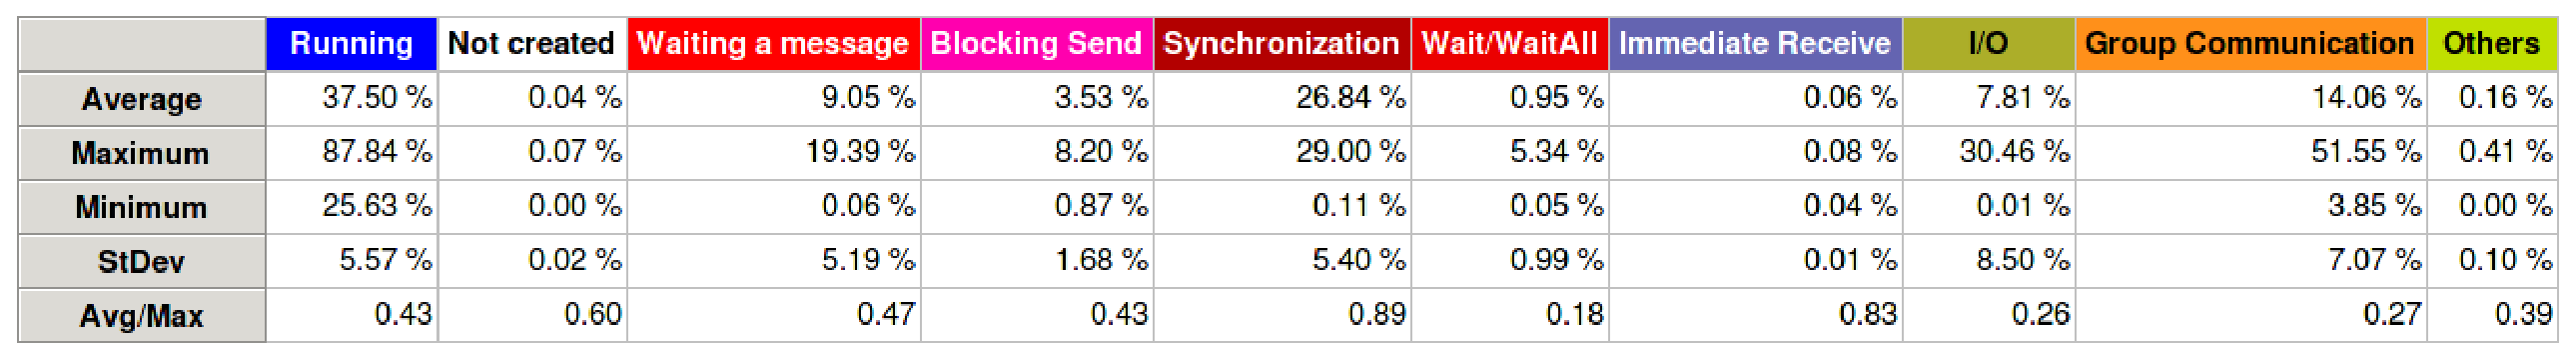
\includegraphics[width=0.78\textwidth]{Figs/23_24_blq0_stat.eps}\\
%   Percentage of time for the 1 hour during midnight (from 23h to 24h) leveraging the polling MPI policy\\
%   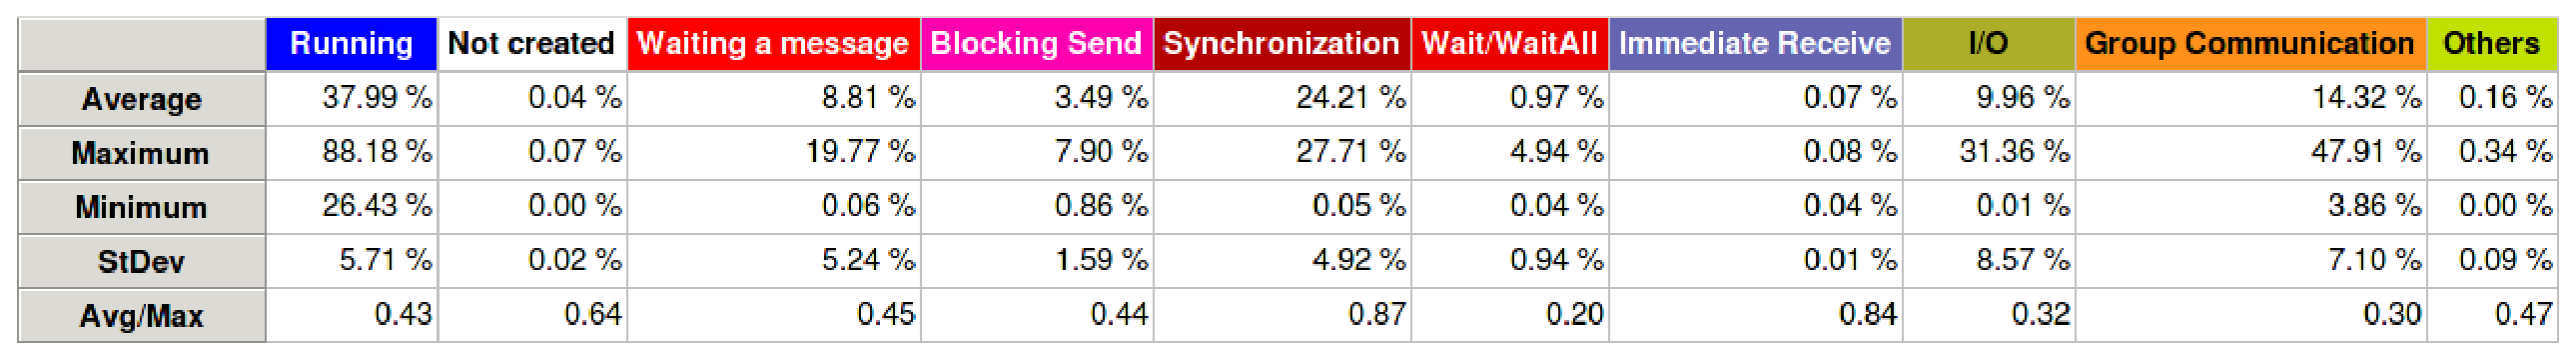
\includegraphics[width=0.78\textwidth]{Figs/23_24_blq1_stat.eps}\\
%   \caption{blabla}
%   \label{fig:8}
% \end{figure*}


\begin{figure*}[ht]
  \centering
  \scriptsize
  Simulation of 1 hour during midday (11h--12h) leveraging the polling MPI policy\\
  \scalebox{0.5}{\input{Figs/11_12_blq0_figure.pstex_t}}\\
  Simulation of 1 hour during midday (11h--12h) leveraging the blocking MPI policy\\
  \scalebox{0.5}{\input{Figs/11_12_blq1_figure.pstex_t}}\\
  1 hour simulation during midnight (23h--24h) leveraging the polling MPI policy\\
  \scalebox{0.5}{\input{Figs/23_24_blq0_figure.pstex_t}}\\
  1 hour simulation during midnight (23h--24h) leveraging the blocking MPI policy\\
  \scalebox{0.5}{\input{Figs/23_24_blq1_figure.pstex_t}}\\
  \begin{tabular}{rlp{-0.2cm}rlp{-0.2cm}rlp{-0.2cm}rlp{-0.2cm}rl}
& &  & &  & &  \\[-0.15cm]
Computation     & \multicolumn{1}{>{\columncolor[RGB]{  0,  , 255}}p{0.4cm}}{}  & & 
Block. send     & \multicolumn{1}{>{\columncolor[RGB]{255,  0,174}}p{0.4cm}}{}  & & 
Synchronization & \multicolumn{1}{>{\columncolor[RGB]{179,  0,  0}}p{0.4cm}}{}  & & 
Wait/Wait all   & \multicolumn{1}{>{\columncolor[RGB]{235,255,  0}}p{0.4cm}}{}  \\
& &  & &  & &  \\[-0.15cm]
Immediate recv. & \multicolumn{1}{>{\columncolor[RGB]{100,100,177}}p{0.4cm}}{}  & &
Waiting a msg.  & \multicolumn{1}{>{\columncolor[RGB]{255,  0  ,0}}p{0.4cm}}{}  & & 
Group comm.     & \multicolumn{1}{>{\columncolor[RGB]{255,144, 26}}p{0.4cm}}{}  & &
Others          & \multicolumn{1}{>{\columncolor[RGB]{192,224,  0}}p{0.4cm}}{}  \\
%I/O             & \multicolumn{1}{>{\columncolor[RGB]{172,174, 41}}p{0.4cm}}{}  & &
%
%Idle            & \multicolumn{1}{>{\columncolor[RGB]{117,195,255}}p{0.4cm}}{}  \\
\end{tabular}
  \caption{Power-performance traces during midday and midnight leveraging the polling and blocking MPI policies on \tinto.}
  \label{fig:11}
\end{figure*}
